\documentclass{article}
\usepackage[UTF8]{ctex}
\usepackage{amsmath,mathtools,geometry,float}

\title{数学改编题}
\author{李俊言}
\date{2024年1月7日}

\begin{document}
已知一块形状不规则的游乐场$ABCDEF$, 其中边$BCD, AFE$均为抛物线, $C$与$F$为顶点, 如图所示. 已知抛物线$BCD$: $y=-2x^2+ax+b$, $AFE$: $y=x^2/2-cx$. 已知点$A:(0,0), B:(1,0), D:(4,0), E:(5,0)$.\par
(1) 求两个抛物线的解析式;\par
(2) 游乐场欲修建一条小火车, 来提高客流运输能力, 同时为游客提供观光服务. 已知游乐场外有两座市政府规划的车站$T:(0,-1)$与$M:(6,4)$. 游乐园负责人在抛物线$BCD$和线段$BD$围成的图形内规划了一座车站$N$, 使得车站$T, B, N$均在一条直线$l$上, 且$S_{\triangle BNC}=\frac{2}{9}S_{\triangle BDC}$. 负责人拟在游乐园边缘另规划一座车站$G$, 使得$\triangle NGM$为直角三角形. 他的设想是否可以实现? 若可以, 请协助他求出所有可能的车站$G$的坐标; 若不可以, 请向他说明理由.\par
(3) 为了以游乐园为支点撬动当地经济发展, 市政府欲规划一个喷泉. 设$P$为游乐园边缘上的动点, 将$P$绕车站$M$顺指针旋转$90^\circ$至$P'$, 市政府欲将$\triangle P'XY$规划为喷泉, 其中$X:(10,15/2)$, $Y:(10,19/2)$, 并且喷泉的面积要达到最大值. 同时, 以$P'$为起点规划一条公路$P'Q$, 其中$Q$在$l$上, 且$\angle P'QB=30^\circ$. 设直线$P'Q$交$x$轴于$R$, 交$y$轴于$S$. 现欲在$l'$上规划一座车站$K$, 在线段$AS$上规划另一座车站$W$使得$\angle AKW=90^\circ$. 取$AW$中点$V$, 连接$KV$. 出于某种考虑, $KV^2/SV$要取到最小值. 请直接写出此时$\triangle SKV$的面积, 精确到小数点后$1$位. 参考值:$\sqrt{2}\approx1.414,\sqrt{3}\approx1.732,\sqrt{6}\approx2.449,\sqrt{10}\approx3.162,\sqrt{17}\approx4.132,\sqrt{31}\approx5.568$
\begin{figure}[H]
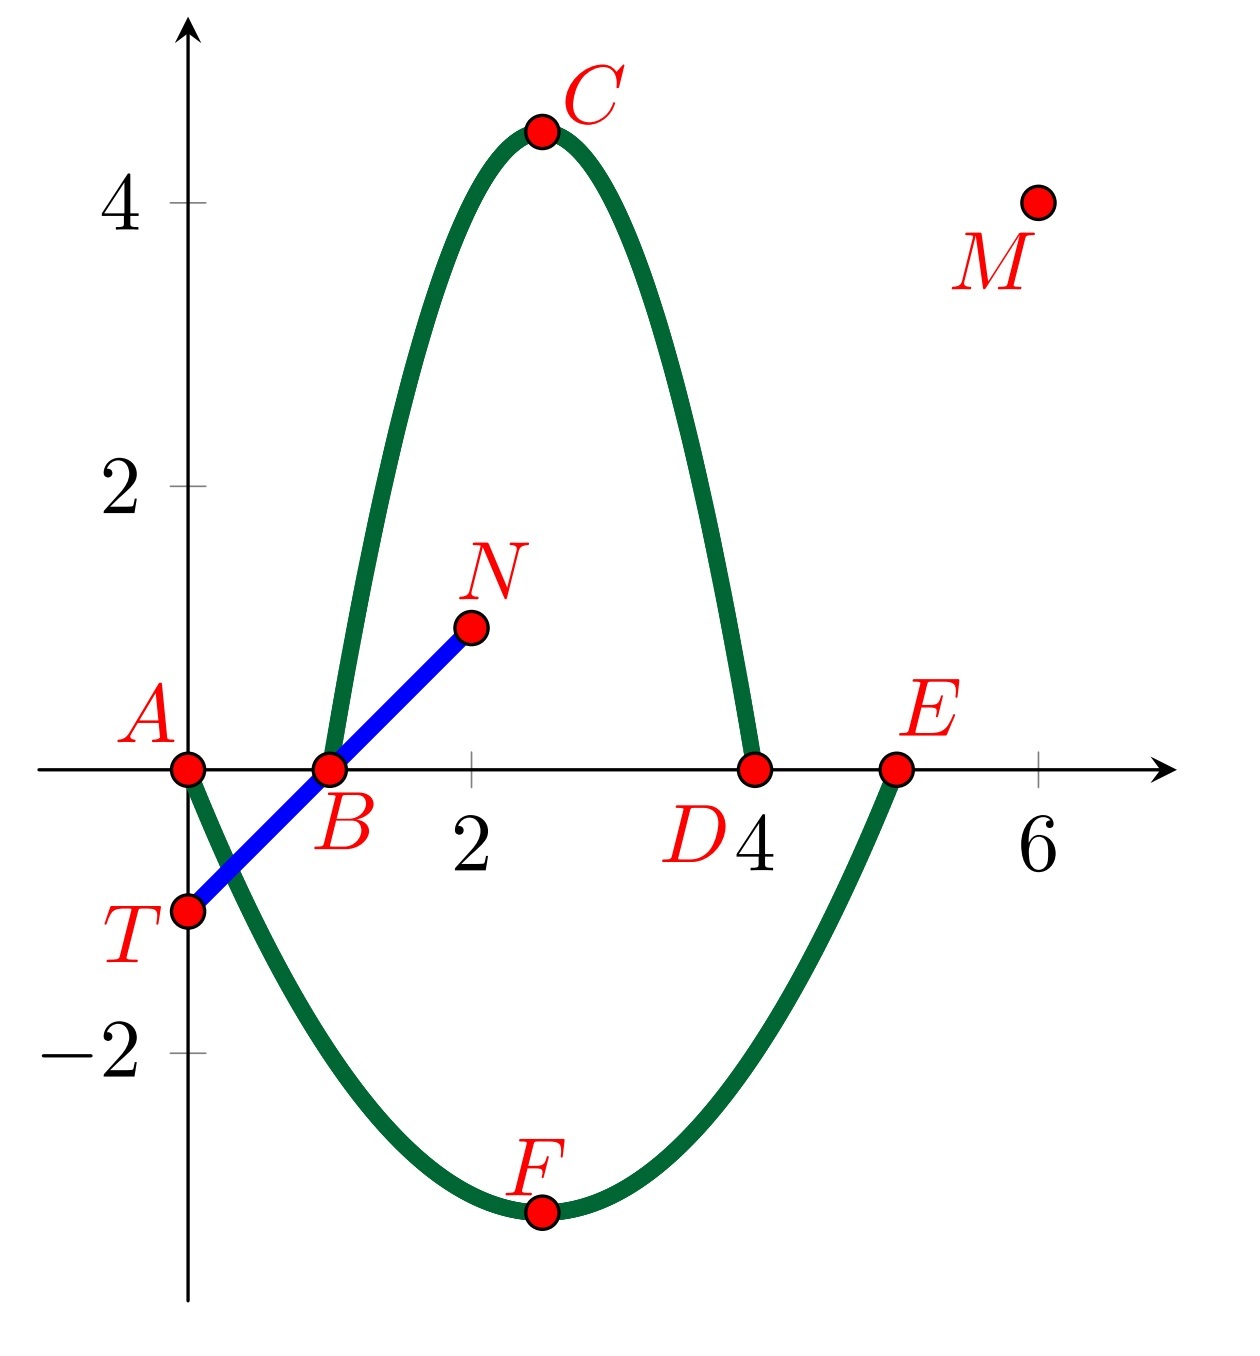
\includegraphics[width=0.4\textwidth]{1.jpg}
\hfill
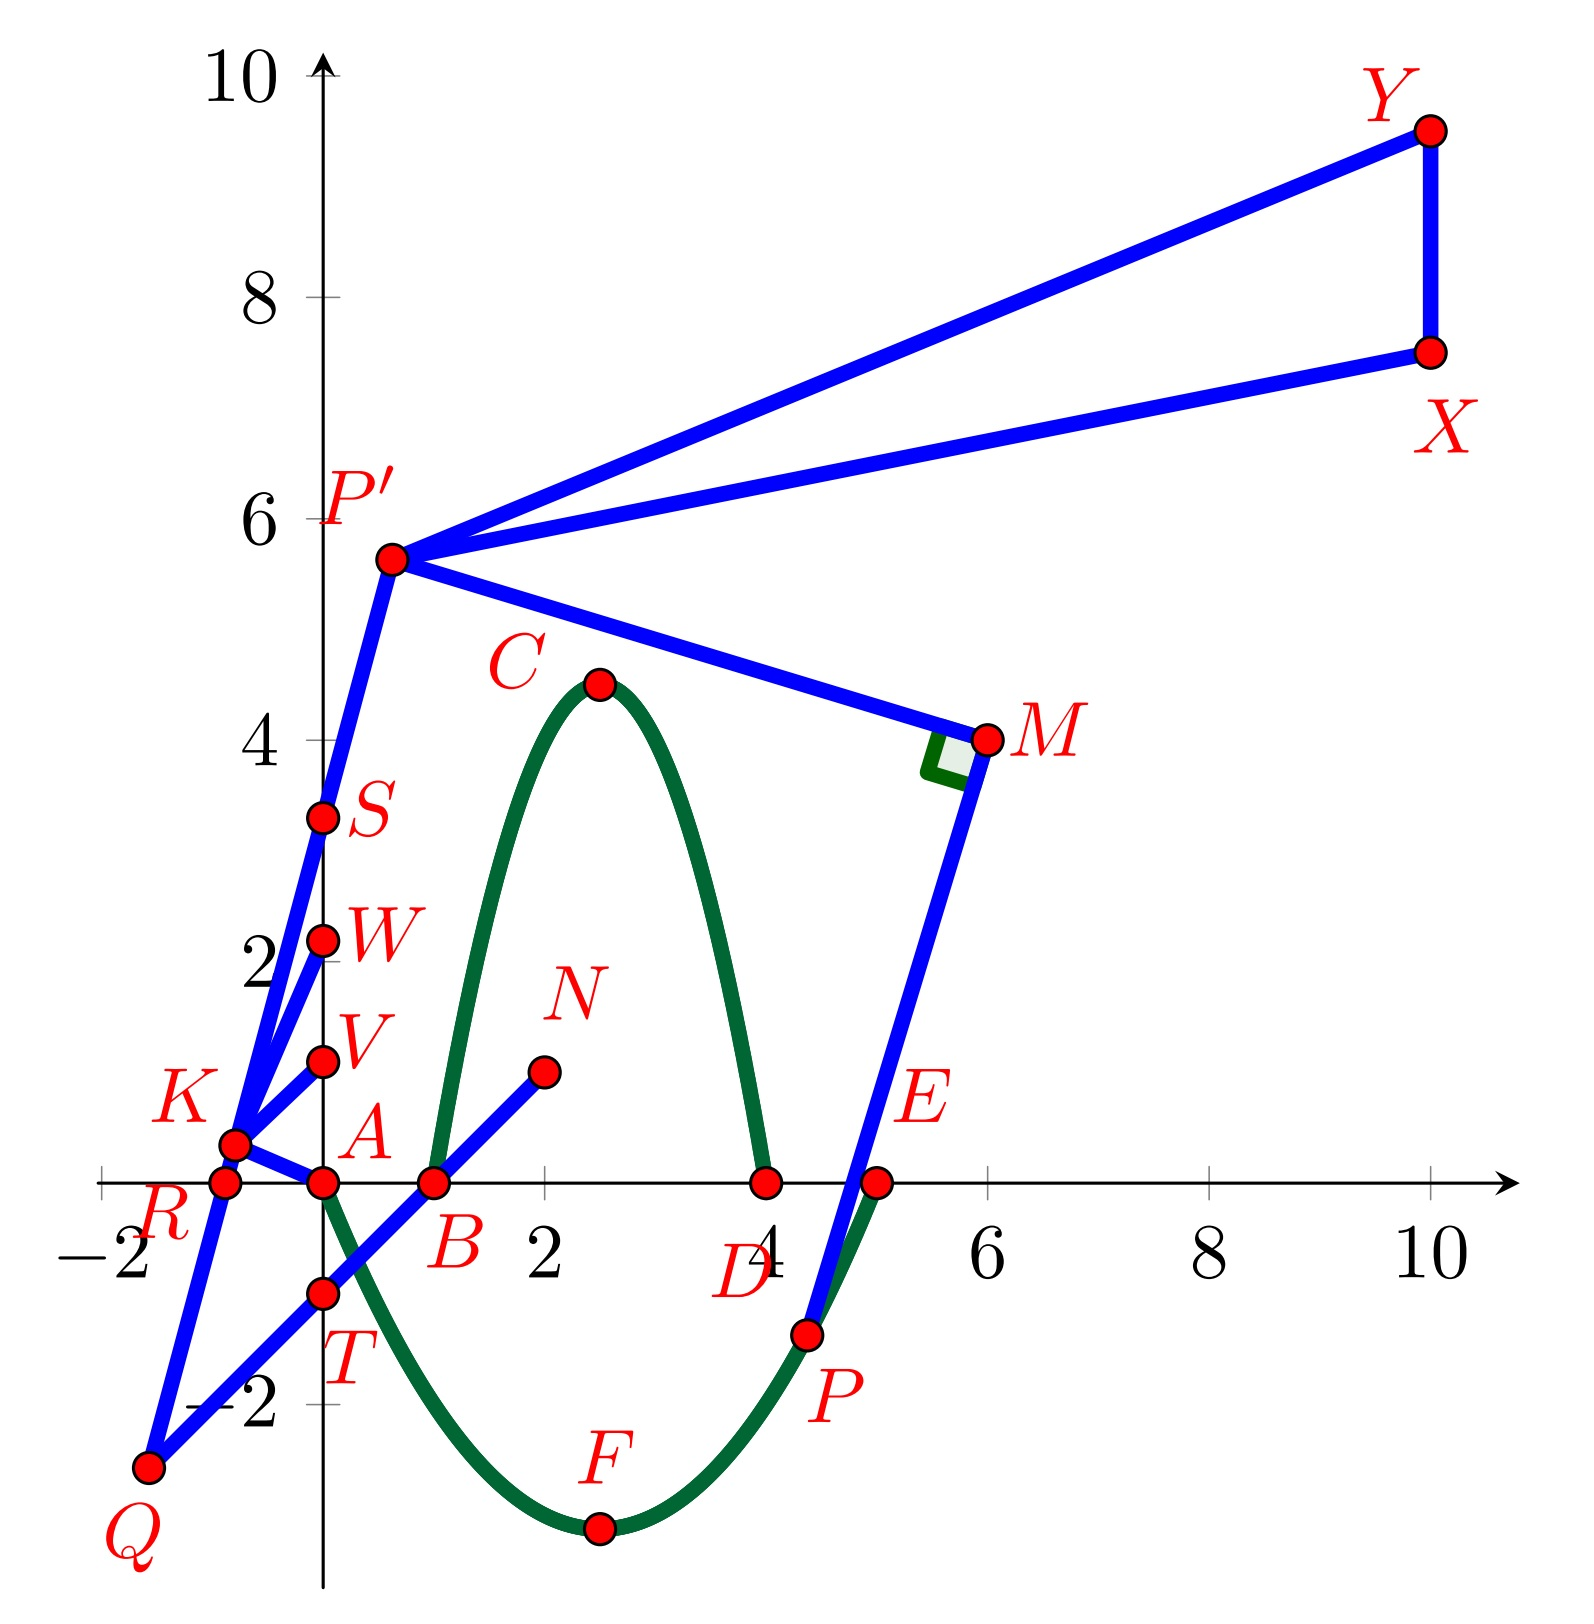
\includegraphics[width=0.59\textwidth]{2.jpg}
\end{figure}
\hspace*{0.15\textwidth}图 1\hfill 图 2\hspace{0.25\textwidth}
\end{document}